

\documentclass[11pt]{article}
%%%%%%%%%%%%%%%%%%%%%%%%%%%%%%%%%%%%%%%%%%%%%%%%%%%%%%%%%%%%%%%%%%%%%%%%%%%%%%%%%%%%%%%%%%%%%%%%%%%%%%%%%%%%%%%%%%%%%%%%%%%%%%%%%%%%%%%%%%%%%%%%%%%%%%%%%%%%%%%%%%%%%%%%%%%%%%%%%%%%%%%%%%%%%%%%%%%%%%%%%%%%%%%%%%%%%%%%%%%%%%%%%%%%%%%%%%%%%%%%%%%%%%%%%%%%
\usepackage{amsmath,amsthm,amssymb, pdfpages,mathtools}
\usepackage{color}
\usepackage{array}
\usepackage{gastex}
\usepackage{subfigure}
\usepackage[normalem]{ulem}
\usepackage{xcolor,psfrag,graphicx}
\usepackage{setspace}
\usepackage{natbib}
\usepackage{lscape}
\usepackage{enumerate}
\usepackage{appendix}
\usepackage[hidelinks, hypertexnames=false]{hyperref}
\usepackage{lscape}

\setcounter{MaxMatrixCols}{10}

\setlength{\evensidemargin}{0.0in}
 \setlength{\oddsidemargin}{0.0in}
 \setlength{\textwidth}{6.5in}
 \topmargin -0.25in
 \textheight 8.5in
 \hfuzz=50pt
 \pagestyle{plain}
\newcommand{\eqthreshn}{{t^*_N}}
\newcommand{\pnd}{1-p+pF(\eqthreshn)}
\newcommand{\ppnd}{\big(1-p+pF(\eqthreshn)\big)}
\newcommand{\eqmfreq}{{\omega^*}}
\newcommand{\eqmfreqn}{{\omega^*_N}}
\newcommand{\eqmfreqnp}{{\omega^*_{N+1}}}
\newcommand{\eqthresh}{{t^*}}
\newcommand{\eqthreshX}{{t^{**}}}
\newcommand{\nbar}{{\overline{N}}}
\newcommand{\wlim}{\omega_\infty}
\newcommand{\wdye}{\hat{\omega}}
\newcommand{\tdye}{\hat{t}}
\newcommand{\limn}{\lim_{N\to\infty}}
\newcommand{\fsn}{\omega_N^*}
\newcommand{\eqprize}{\phi^*}
\newcommand{\moprize}{\phi^M}
\newcommand{\dif}{\;\mathrm{d}}
\newcommand{\diffp}[2]{\frac{\partial #1}{\partial #2}}
\newcommand{\diff}[2]{\frac{\dif #1}{\dif #2}}
\renewcommand{\Re}{\mathbb{R}}                             
\def\endproof{{\quad}$\blacksquare$}
\newcommand{\indicator}[1]{\mathbbm{1}_{\left[ {#1} \right]}}
\newtheorem{theorem}{Theorem}
\newtheorem{proposition}{Proposition}
\newtheorem{prop}{Proposition}
\newtheorem{example}{Example}
\newtheorem{assumption}{Assumption}
\newtheorem{corollary}[theorem]{Corollary}
\newtheorem{acknowledgement}[theorem]{Acknowledgement}
\newtheorem{definition}{Definition}
\newtheorem{lemma}{Lemma}
\newtheorem{remark}{Remark}
\newtheorem{condition}[theorem]{Condition}
 \setlength{\evensidemargin}{0.0in}
 \setlength{\oddsidemargin}{0.0in}
 \setlength{\textwidth}{6.5in}
 \topmargin -0.25in
 \textheight 8.5in
 \hfuzz=50pt
 \pagestyle{plain}
\newcommand{\Change}[1]{{\color{red}#1}}
\renewcommand{\theenumi}{\roman{enumi}}            
\renewcommand{\labelenumi}{(\theenumi)}

%%%%%%%%%%%%%%%
% Page Format %
%%%%%%%%%%%%%%%
 \setlength{\evensidemargin}{0.0in}
 \setlength{\oddsidemargin}{0.0in}
 \setlength{\textwidth}{6.5in}
 \topmargin -0.25in
 \textheight 8.5in
 \hfuzz=50pt
 \pagestyle{plain}





\begin{document}
\title{\textbf{TV Identities: \\ TITLE}%Unravel}
\thanks{We would like to thank XYZ.}\\
}



\author{Andrew Kao\thanks{University of Chicago, andrewkao@uchicago.edu.} }

%\begin{center}
\date{January 2020}
{\vspace{-5ex}}
%\end{center}


\maketitle

\begin{abstract}
%\noindent When deciding whether to publicly express their views and attitudes, individuals may take into account their perception of the social acceptability of these views, which in turn depends on (and affects) their perception of the popularity of the view. Even if a substantial fraction of society \emph{privately} holds a specific view, that view might end up stigmatized and publicly withheld in equilibrium if individuals have initial beliefs that the view is stigmatized. 

%%%% FOR SUBMISSION FORM:
%\noindent Social norms, usually persistent, can unravel quickly when new public information arrives, such as surprising election outcomes. In our model of strategic communication, senders state their opinion but they can lie to pander to the popular view; receivers thus make less inference about such senders. We test the model's predictions with two experiments. On the sender's side, we show that Trump's rise in popularity and eventual victory increased individuals' willingness to publicly express xenophobic views. On the receiver's side, we show that individuals are judged less if they expressed a xenophobic view in an environment where the view is popular.


\noindent Here's an abstract
\noindent
\\
%\textbf{JEL Codes:} D1, I31, Z13.\\
%\textbf{Keywords:} 
\end{abstract}




\newsavebox{\tablebox} \newlength{\tableboxwidth}

\setlength{\baselineskip}{22pt}

\renewcommand{\thefootnote}{\fnsymbol{footnote}}


\thispagestyle{empty}

\newpage 
\renewcommand{\thefootnote}{\arabic{footnote}}

\pagebreak 
\setcounter{page}{0}


\onehalfspacing

%\tableofcontents

\newpage

\setcounter{page}{1}
\section{Introduction}

Mass media lets us know what the outside world thinks, and this shapes the way that we think.

- Media plays a large role in shaping our lives

- Latino consumption of broadcast TV remains relevant

- Relevant subquestion: how identity is affected

Three domains

- Education

- Firms

- Politics


The high level research question is to look at the effect of reinforcing identity within Hispanic populations on their schooling outcomes. Specifically, I'll be using the influence of Spanish language television as the channel by which identity is reinforced, and look at how it affects everything from graduation rates to disciplinary action taken to math abilities and English proficiency for Hispanic students in public schools. In short, if I have access to more programming from my home country, does this make me less engaged in school (perhaps because there are more distractions or because it socially ostracizes me etc.), or does this make me perform better (perhaps because l have more role models or because I have something to talk with peers about in school, and hence motivation to attend/perform)?

There's good reason to believe that identity, as reinforced through mass media, has a large effect on the lives people lead.   Oberholzer-Gee, Waldfogel (AER 2009) demonstrate that the presence of Spanish language local news increases Hispanic voter turnout, while Yanigazawa-Drott (QJE 2014) shows that radio broadcasts in Rwanda contributed to the violence and genocide that took place in the 90s. It would be reasonable to think then, that there could be a meaningful effect of Spanish language TV on education. 

%Social norms are an important element of any society: some behaviors and opinions are socially desirable, while others are stigmatized. There is growing evidence that individuals care to a large extent about how they are perceived by others and that such concerns might affect important decisions in a variety of settings

% viewed by half of all Spanish-dominant Latinos (http://www.horowitzresearch.com/press/spanish-language-tv-content-remains-integral-to-u-s-hispanics-tv-diet-new-horowitz-survey-shows/)
% better: Nielsen, 78% Spanish-dominant watch Spanish TV, 50% in multi-language homes, over 85% broadcast -- in 2010, top 10 broadcast shows in Hispanic demographic were all Spanish language
% market size: millions in LA, New York etc. https://www.statista.com/statistics/189824/largest-hispanic-television-markets-in-the-united-states-2011/

% broadcast/satellite TV vs cable: https://www.quora.com/What-is-the-difference-between-cable-and-broadcast

% in recent years, highest viewed: Peque�os Gigantes (talent show, kids), El Se�or de los Cielos (telenovella, cartel leader),   https://www.statista.com/statistics/497739/spanish-tv-programs-usa/

% \citep{andreoni_bernheim_2009, dellavigna_list_malmendier_2012_testing_altruism, andreoni_rao_trachtman_2017} to schooling choices (\citealp{bursztyn_jensen_2015_peer_education}) to political behavior (\citealp{gerber_green_larimer_2008, dellavigna_list_malmendier_rao_2017_voting, enikolopov_makarin_petrova_plishchuk_2017_social_image, ricardo_cruces_2017}). 

%\footnote{% We thus focus on the consequences of Trump's election rather than its causes or
%determinants. With respect to the latter, \citet{enke_2017_trump}
%demonstrates the link between tribalistic (as opposed to universal) moral
%values and Trump vote at the county level, while %
%\citet{allcott_gentzkow_2017_fake_news} discuss the possible role of fake
%news. Relatedly, \citet{xiong_2017_personality} studies the effect of the
%celebrity status of Ronald Reagan on his electoral support, and suggests
%that a similar effect may have helped Trump. At the same time, our focus is
%on causes and not consequences of changes in social norms (see %
%\citealp{ali_benabou_2016}, on the latter).}

%% Do everything with d^2
%% spatial errors: http://www.trfetzer.com/using-r-to-estimate-spatial-hac-errors-per-conley/



%% FOR LATER
% \section{Model/Background/Hypothesis}\label{sectheory}



\section{Data}\label{secdata}

Overall data and brief explanation of sources

Data for the instrument comes from both the FCC and TMS (a telecommunications company that was kind enough to let me use their API for free), and the instrument is fully constructed. The relevant data here is essentially just the coverage contour spatial data and the broadcast language of the station.

The data on public schools comes from the US government's CRDC (Civil Rights Data Collection) dataset. It's a very large dataset with a ton of outcome/control variables, but importantly, it breaks down all major variables of interest by ethnicity. These variables includes graduation rates, chronic absenteeism, suspensions, expulsions, arrests, bullying, AP test results, English proficiency, math class performances, gifted program enrolment etc., so I can look at effects on both the top and bottom end of the distribution, and examine potential mechanisms driving outcomes. These are all at the school level, and so I can run this through ArcGIS to get physical locations of these schools as well.

I get additional controls for things like population, income, density of Hispanic population etc. at the county level from IPUMS.

\subsection{Broadcast TV}


\subsection{Outcomes}


% Table created by stargazer v.5.2.2 by Marek Hlavac, Harvard University. E-mail: hlavac at fas.harvard.edu
% Date and time: Fri, Dec 13, 2019 - 20:45:59
\begin{table}[!htbp] \centering 
  \caption{School-District Level Summary Statistics} 
  \label{} 
\begin{tabular}{@{\extracolsep{5pt}}lccccccc} 
\\[-1.8ex]\hline 
\hline \\[-1.8ex] 
Statistic & \multicolumn{1}{c}{N} & \multicolumn{1}{c}{Mean} & \multicolumn{1}{c}{St. Dev.} & \multicolumn{1}{c}{Min} & \multicolumn{1}{c}{Pctl(25)} & \multicolumn{1}{c}{Pctl(75)} & \multicolumn{1}{c}{Max} \\ 
\hline \\[-1.8ex] 
Distance to Boundary & 17,280 & 136.855 & 146.751 & 0.000 & 15.786 & 217.567 & 806.543 \\ 
SLTV Coverage Dummy & 17,280 & 0.292 & 0.455 & 0.000 & 0.000 & 1.000 & 1.000 \\ 
\% County Hispanic & 17,280 & 7.051 & 11.950 & 0.000 & 0.668 & 6.974 & 97.216 \\ 
Log(Population) & 17,280 & 11.618 & 1.840 & 5.869 & 10.242 & 13.110 & 15.997 \\ 
Log(Income) & 17,280 & 9.428 & 0.257 & 7.976 & 9.257 & 9.593 & 10.245 \\ 
\hline \\[-1.8ex] 
\multicolumn{8}{l}{\textit{Note:} Distance to SLTV Boundary measured in KM} \\ 
\end{tabular} 
\end{table} 


% Table created by stargazer v.5.2.2 by Marek Hlavac, Harvard University. E-mail: hlavac at fas.harvard.edu
% Date and time: Fri, Dec 13, 2019 - 22:32:28
\begin{table}[!htbp] \centering 
  \caption{School Level Summary Statistics} 
  \label{} 
\begin{tabular}{@{\extracolsep{5pt}}lccccccc} 
\\[-1.8ex]\hline 
\hline \\[-1.8ex] 
Statistic & \multicolumn{1}{c}{N} & \multicolumn{1}{c}{Mean} & \multicolumn{1}{c}{St. Dev.} & \multicolumn{1}{c}{Min} & \multicolumn{1}{c}{Pctl(25)} & \multicolumn{1}{c}{Pctl(75)} & \multicolumn{1}{c}{Max} \\ 
\hline \\[-1.8ex] 
Total Students & 96,349 & 524.859 & 449.354 & 2.000 & 254.000 & 662.000 & 14,164.000 \\ 
\# Hispanic Students & 91,019 & 143.195 & 243.873 & 2.000 & 13.000 & 166.000 & 7,675.000 \\ 
Contains Grade 1 & 96,350 & 0.538 & 0.499 & 0 & 0 & 1 & 1 \\ 
Contains Grade 6 & 96,350 & 0.364 & 0.481 & 0 & 0 & 1 & 1 \\ 
Contains Grade 9 & 96,350 & 0.253 & 0.435 & 0 & 0 & 1 & 1 \\ 
Hispanic Suspension Dummy & 94,535 & 0.382 & 0.486 & 0.000 & 0.000 & 1.000 & 1.000 \\ 
Hispanic Chronic Absentees & 94,540 & 22.920 & 57.838 & 0.000 & 0.000 & 22.000 & 2,131.000 \\ 
\# Teachers & 93,934 & 35.219 & 33.892 & 1.000 & 19.000 & 44.000 & 6,031.000 \\ 
\hline \\[-1.8ex] 
\multicolumn{8}{l}{\textit{Note:} Dummies indicate whether event occurred in the school over the past year} \\ 
\end{tabular} 
\end{table} 




\section{Empirical Strategy}\label{secrd}

To isolate the causal effect of Spanish language television, I adopt the technique used in \citep{velez_tuning_2019} Newman, Velez (AJPS 2019) and generalize it from three counties to the entirety of the US. Newman and Velez exploit a FCC (Federal Communications Commission) regulation which determines the distance from a TV station in which the station's broadcast signal is protected from interference. This creates a natural regression discontinuity, where the decaying strength of a signal over distance is combined with this cutoff in broadcast protection to create a split among people just inside and outside these coverage 'contours' that are presumably comparable save for their access to broadcast TV. 

In the case of Spanish language TV in particular, this should allow me to examine its causal effect on Hispanic populations for spatially located outcomes, such as public schooling results. It's worth noting that these contours are purely determined by an algorithm that looks at things like local elevation and antennae strength, so that the cutoffs are located in more or less random locations, and that coverage is large enough that these contours tend to cut across towns and suburbs, rather than cities. Finally, regressions using US census data indicate that Hispanic people do not migrate across counties in response to these contours.

A standard regression thus looks like restricting the universe of schools to only those within a small radius of the contour boundary, where the key independent variable of interest is an indicator for the school being inside or outside the boundary.

\subsection{Main Specification}

A standard regression thus looks like restricting the universe of schools to only those within a small radius of the contour boundary, where the key independent variable of interest is an indicator for the school being inside or outside the boundary, interacted with the distance to the boundary:
\[ Y_i^{j,k} = \beta_0 + \beta \mathbb{I}[InsideContour_i] \times Distance_i + \gamma X_i + \delta Z^j + \epsilon_i^k \, \, \, \, \, \, \, \epsilon \stackrel{iid}{\sim}   N(0,\sigma_i^{k^2})\]

where $Y_i$ is an outcome for school $i$ in county $j$ and school district $k$, $X$ is a vector of school-level controls, and $Z$ is a vector of county-level controls. Errors are often clustered by school district, meaning that $Corr(\sigma_i^k, \sigma_{i'}^k) \neq 0$ is permissible.

By limiting the analysis to a small distance from the contour boundary ($100$ KM/63 miles by default), we also minimize the potential concerns of omitted variable bias etc., as these schools must now be at least fairly close to one another, meaning that they probably share many overarching characteristics.


\subsection{Migration}

\section{Public Schools}\label{secschool}
\subsection{Data}
\subsection{Results}
\subsection{Discussion}
\paragraph{Evidence of Mechanism}
Targeting based on identity

\section{Firms}\label{secfirm}
\subsection{Data}
\subsection{Results}
\subsection{Discussion}

\section{Campaign Contributions}\label{seccamp}
\subsection{Data}
\subsection{Results}
\paragraph{Wave 1: Intervention Before the Election.}
% Univision and Telemundo emphasize their lineups of telenovelas, sports and reality programming.
% Reasons for Trump: (1) broadcasts in SLTV lean conservative, reflect conservative values, (2) legal immigration, (3) news might lean conservative: https://www.nytimes.com/2012/08/13/business/media/mundofox-new-spanish-language-network-to-make-debut.html
% contrary to public opinion: https://www.npr.org/sections/itsallpolitics/2014/04/01/297827352/conservative-media-watchdog-univision-telemundo-favor-liberals
% https://foreignpolicy.com/2018/04/16/the-trumpification-of-the-latin-american-right/
\subsection{Discussion}



%We implemented the first experiment respectively in the two weeks before and in the week after the 2016 presidential election. The timing of the experiment allowed us to exploit the uniqueness of the situation and study the process of information aggregation as it was unfolding. We conducted both waves with workers from the online platform MTurk. A number of recent papers in economics have used the same platform to conduct surveys or experiments (e.g., \citealp{kuziemco_et_al_2015_elastic}). The platform draws workers from very diverse backgrounds, though it is not representative of the U.S. population as a whole.


%Appendix Table \ref{balance1} provides evidence that individual characteristics are balanced across all four pre-election experimental conditions, confirming that the randomization was successful. The first four bars of Figure \ref{mainexperiment1fig} display our main findings from the pre-election experiment. In the control condition before the election, we observe a large and statistically significant wedge between donation rates in private and in public: a drop from 54\% in private to 34\% in public (the p-value of a \emph{t} test of equality is 0.002). Among individuals in the information condition, we observe no difference in private and public donation rates, which are 47\% and 46\%, respectively (\emph{p}-value=0.839). Moreover, we find no significant difference in private donation rates between the information and control conditions (\emph{p}-value=0.280), suggesting that the information is not increasing privately-held xenophobia. The increase in public donation rates between the two conditions is statistically significant (\emph{p}-value=0.089), as is the difference in differences between donation rates in private across conditions and donation rates in public across conditions (\emph{p}-value=0.050). These results indicate that the information provided causally increased the social acceptability of the action to the point of eliminating the original social stigma associated with it.\footnote{Apart from social stigma, another possible reason %An additional explanation to social stigma 
%for the lower donation rates in the public condition with respect to the private condition is that participants might want to avoid talking with the surveyor because of the extra effort and time this requires (independently of the topic of the conversation), and they might expect the likelihood of having to talk to be higher in case they decide to make the donation. However, this mechanism should operate identically both in the control and in the treatment conditions, thus not affecting our identification of the reduction in social stigma.} The first two columns of Table \ref{mainexperiment1tab} display the difference in differences results in regression format and show that our results are unchanged when individual covariates are included. The table also displays \emph{p}-values from permutation tests, showing that our findings are robust to that inference method.




\section{Conclusion} \label{secconcl}


\clearpage
\pagebreak

\begin{singlespace}
%\bibliographystyle{aea}
\bibliographystyle{plainnat}
\bibliography{tv_bib.bib}
abc
\end{singlespace}

\pagebreak
\clearpage

\section*{Figures and Tables}

%%%%%%%%%%%%%%%%%%%%%%%%%%%%%%%%%
% Figure 1: Coverage Contours
%%%%%%%%%%%%%%%%%%%%%%%%%%%%%%%%%

\begin{figure}[!hbtp]
\centering
\caption{The Coverage Contours of Spanish Language TV stations}\label{contourfig}
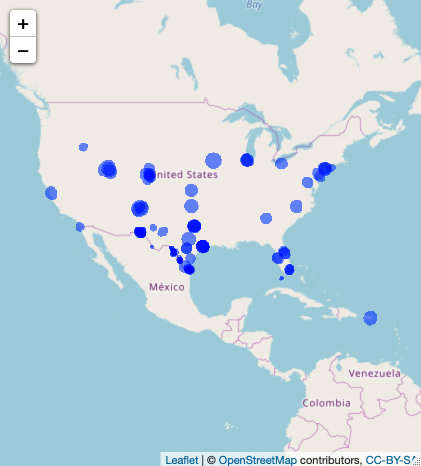
\includegraphics[width=8cm]{../../analysis/Output/img/SpanishContours.png}
\end{figure} 

\begin{figure}[!hbtp]
\centering
\caption{Map of School Districts in the US}\label{schooldistrictfig}
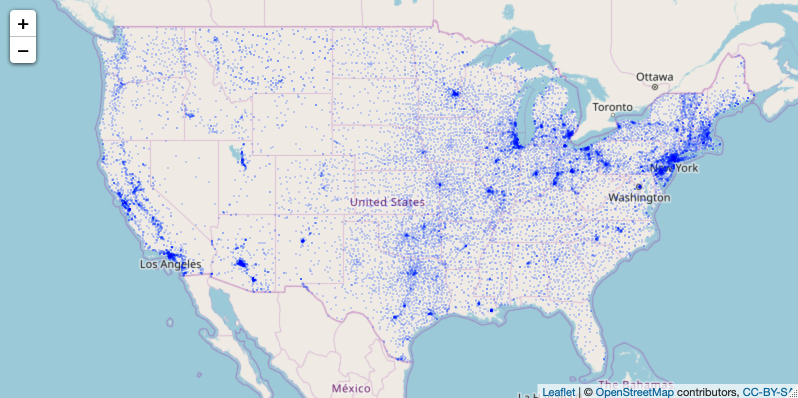
\includegraphics[width=12cm]{../../analysis/Output/img/LEAMap.png}
\end{figure} 

%\begin{figure}[!h]
%\begin{center}
%\caption{{\bf Proposition 3: Receiver's Priors and Posteriors}} \label{theoryfig1}
%
%\
%
%\includegraphics[scale=.35]{Figure1Updated.pdf}
%
%\end{center}
%\end{figure}

%\begin{figure}[!h]
%\begin{center}
%\caption{{\bf Experiment 1A: Donation Rates Before and After the Election}} \label{mainexperiment1fig}
%
%\
%
%\includegraphics[scale=1]{fig_1_2017.eps}
%
%\settowidth{\tableboxwidth}{\usebox{\tablebox}} \parbox{.92\textwidth}
%{\emph{Notes}: the two bars on the left display donation rates to the anti-immigration organization for individuals in the private and public conditions in the control group before the election (full sample, respectively N=112 and N=111), the two central bars display those in the information group before the election (full sample, respectively N=102 and N=103), and the last two bars display those in the control group after the election (for individuals already surveyed before the election, respectively N=82 and N=84). Error bars reflect 95\% confidence intervals. Top horizontal bars show \emph{p}-values for \emph{t} tests of equality of means between different experimental conditions.}
%\end{center}
%\end{figure}

\pagebreak



%\begin{table}[!h]
%  \centering
%\caption{{\bf Experiment 1A: Difference in Differences Regressions}\label{mainexperiment1tab}} 
%      \begin{lrbox}{\tablebox}
%\begin{tabular}{l*{4}{c}}
%\\
%\hline
%            Dependent&\multicolumn{4}{l}{Dummy: individual authorizes donation to}\\
%                        Variable&\multicolumn{4}{l}{anti-immigrant  organization}\\
%\hline
%            &\multicolumn{1}{c}{(1)}&\multicolumn{1}{c}{(2)}&\multicolumn{1}{c}{(3)}&\multicolumn{1}{c}{(4)}\\
%\hline
%Public & -0.202*** & -0.200*** & -0.202*** & -0.199***\\
%& [0.065] & [0.066] & [0.065] & [0.065]\\
%& (0.004) & (0.005) & (0.004) & (0.007)\\
%Information & -0.074 & -0.077 & -0.074 & -0.076\\
%& [0.069] & [0.068] & [0.069] & [0.068]\\
%& (0.277) & (0.266) & (0.277) & (0.281)\\
%Public*Information & 0.188* & 0.178* & 0.188* & 0.178*\\
%& [0.096] & [0.096] & [0.096] & [0.096]\\
%& (0.045) & (0.062) & (0.045) & (0.062)\\
%After Election & & & -0.057 & -0.062\\
%& & & [0.073] & [0.072]\\
%& & & (0.380) & (0.304)\\
%Public*After Election & & & 0.191* & 0.186*\\
%& & & [0.102] & [0.101]\\
%& & & (0.071) & (0.080)\\
%Mean Donation Rate\\
%Control Private & \multicolumn{4}{c}{0.545}\\
%Before Election\\
%\hline
%Controls & No & Yes & No & Yes\\
%N & 428 & 428 & 594 & 594\\
%$R^{2}$ & 0.022 & 0.033 & 0.017 & 0.034\\
%\hline
%\end{tabular}
%   \end{lrbox}
%
%   \usebox{\tablebox}\\
%\settowidth{\tableboxwidth}{\usebox{\tablebox}} \parbox{.995\tableboxwidth}{\emph{Notes}: Columns (1) and (2) includes the full pre-election sample. Columns (3) and (4) add the post-election sample of individuals already surveyed before the election. Columns (1) presents OLS regression of a dummy variable for whether a individual donates to the anti-immigration organization on a dummy for the Public condition, a dummy for the Information condition, and a dummy for the Public Information condition. The control private condition before the election is the omitted group, for which we report the mean donation rate. Columns (3) replicates and adds a dummy for the after election condition, and a dummy for the Public after election condition. Columns (2) and (4) replicate and add individual covariates (gender, age, marital status, years of education, household income, and race). Robust standard errors in brackets. \emph{P}-values from permutation tests with 1,000 repetitions in parentheses. * significant at 10\%; ** significant at 5\%; *** significant at 1\% based on robust standard errors.}
%%\end{tiny}
%\end{table}
%

\end{document}

